%!TEX root = ../thesis.tex

\section{実験要件}
実験には下記のコンピュータとソフトウェアを用いた. 

\begin{enumerate}
  \item コンピュータ\\
  OS: Ubuntu 20.04 LTS\\
  ROS: Noetic\\
  CPU: intel Core i7-10700F(4.8GHz/8コア/16スレッド)\\
  DRAM: 32GB DDR4(3200/8GB×4)
  \item nav\_cloning(学習器, 統合環境)\\
  \url{https://github.com/open-rdc/nav_cloning}
  \item waypoint\_nav(移動目標地点, 目標方向を出力)\\
  \url{https://github.com/open-rdc/waypoint_nav}
  \newpage
  \item turtlebot3 関連\\
  \url{https://github.com/open-rdc/turtlebot3}
  \item navigation(ナビゲーションパッケージ)\\
  \url{https://github.com/ros-planning/navigation}
\end{enumerate}

\subsection{実験装置(シミュレータ)}

\begin{itemize}
  \item ロボット

ロボットモデルは前報\cite{okada1}\cite{okada2}と同様, \figref{Fig:waffle_pi}に示すように, TurtleBot3 Waffle\_piへ3つのカメラを追加したモデルを用いる.

\begin{figure}[hbtp]
  \centering
 \includegraphics[keepaspectratio, scale=0.22]
      {images/Waffle_pi.png}
 \caption{TurtleBot3 waffle\_pi with 3 cameras}
 \label{Fig:waffle_pi}
\end{figure}

\item 環境\\
シミュレータ環境として, オープンソースの3DロボットシミュレータGazeboを用いる. \figref{Fig:sim}に示すようなGazebo上で千葉工業大学2号館3階を模した実験環境を対象に実験を行う.

\begin{figure}[hbtp]
  \centering
 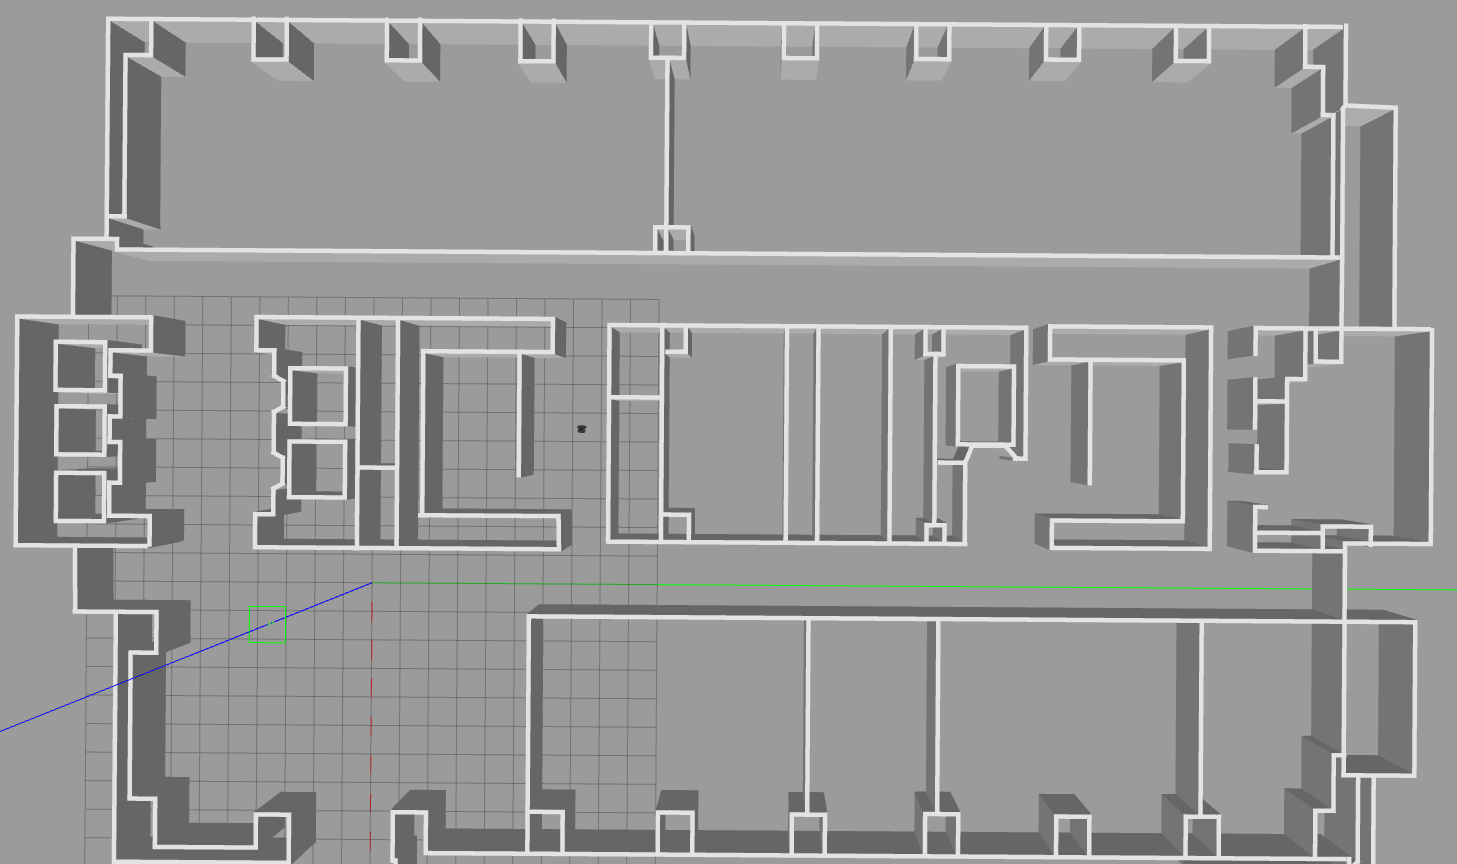
\includegraphics[keepaspectratio, scale=0.12]
      {images/tsudanuma2-3_simorg.png}
 \caption{Experimental enviroment of simulator}
 \label{Fig:sim}
\end{figure}

\end{itemize}

\subsection{実験方法}
\figref{Fig:sim_explain}のA, B地点において, \figref{Fig:select}に示すように侵入する方向が3つあり, 進むことのできる方向が2つあることから, 1箇所につき走行パターンが6つ存在する. 
また, A, B地点では, 目標方向に従って任意の経路を選択することが求められる場所である.
したがって, 実験ではA, B地点で合計12パターンの走行において, 与えた目標方向に従った行動が行えるのかを確認する.

\begin{figure}[hbtp]
  \centering
 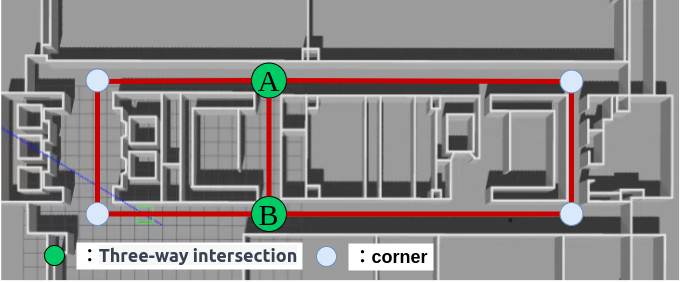
\includegraphics[keepaspectratio, scale=0.5]
      {images/sim_explain.png}
 \caption{Characteristics of passages in the experimental environment on the simulator}
 \label{Fig:sim_explain}
\end{figure}

\begin{figure}[hbtp]
  \centering
 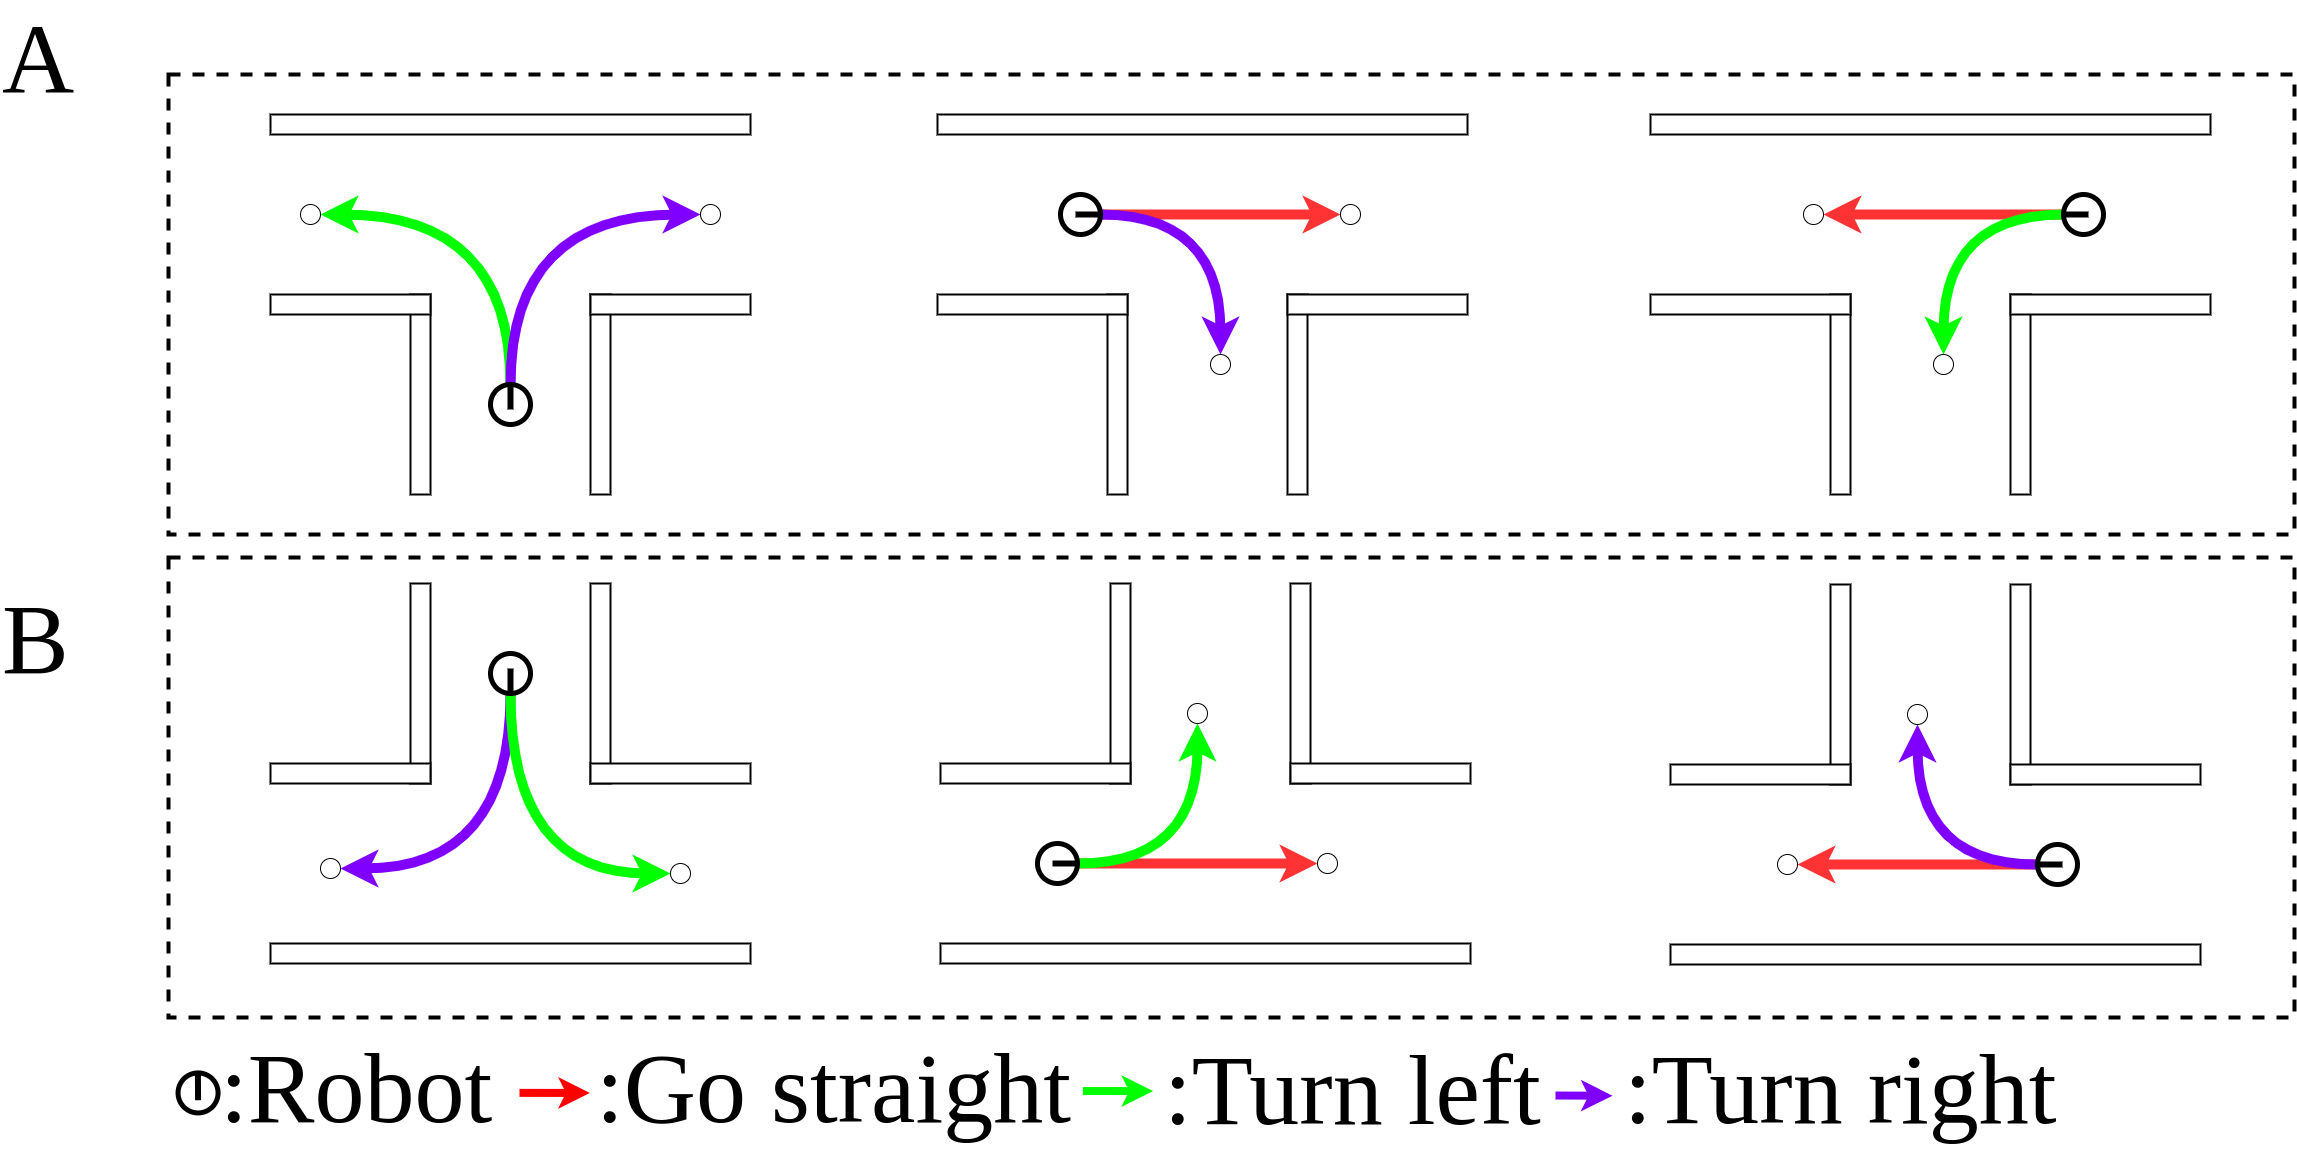
\includegraphics[keepaspectratio, scale=0.15]
      {images/select.png}
 \caption{Moving pattern at points A and B}
 \label{Fig:select}
\end{figure}

ほこ\\
ころ

\begin{figure}[hbtp]
  \centering
 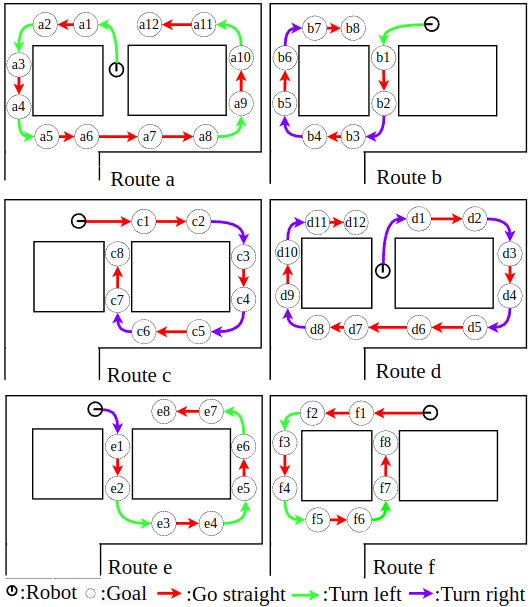
\includegraphics[keepaspectratio, scale=0.6]
      {images/route.png}
 \caption{Moving pattern at points A and B}
 \label{Fig:route}
\end{figure}

\newpage
